\documentclass{emulateapj}
\bibliographystyle{apj}

%define general packages
\usepackage{epsfig}
\usepackage{rotating}
\usepackage{amsmath}
\usepackage{footnote}
\usepackage{setspace}
\usepackage{courier}


\begin{document}

\title{Fiber Collision Correction Method for BOSS Power Spectrum} 

\author{ChangHoon~Hahn\altaffilmark{1}, 
Michael R.~Blanton\altaffilmark{1}, 
Roman~Scoccimarro\altaffilmark{1}} 
\altaffiltext{1}{Center for Cosmology and Particle Physics, Department of Physics, New York University, 4 Washington Place, New York, NY 10003; chh327@nyu.edu}

\begin{abstract}
Redshift surveys, including BOSS, use fiber fed spectrographs. A fiber is used for each galaxy in order obtain its redshift. However, due to the physical size of the fibers, if galaxies are located in close proximity to each other on the sky (not necessary along the line-of-sight) two separate fibers cannot be placed adjacently in order to separately extra the spectroscopic information. In such a scenario, the redshift of fiber-collided galaxies are not individually resolved and only a single redshift for them can be calculated. Though this only accounts for $< 5\%$ of the BOSS redshift survey, its effect on the statistical measures such as the powerspectrum and bispectrum is sufficient in small scales to warrant a detailed correction scheme.
\end{abstract}
\keywords{cosmology: observations --- }


\section{Introduction} 
\begin{itemize}
\item fiber-fed multi-object spectroscopic surveys allow us to collect large redshift data, which is why it?s the favorite of cosmology surveys
\item moving from statistics dominated regime to systematics dominated regime
\end{itemize}

Redshift surveys, including BOSS, use fiber fed spectrographs. A fiber is used for each galaxy in order obtain its redshift. However, due to the physical size of the fibers, if galaxies are located in close proximity to each other on the sky (not necessary along the line-of-sight) two separate fibers cannot be placed adjacently in order to separately extra the spectroscopic information. In such a scenario, the redshift of fiber-collided galaxies are not individually resolved and only a single redshift for them can be calculated. Though this only accounts for $< 5\%$ of the BOSS redshift survey, its effect on the statistical measures such as the powerspectrum and bispectrum is sufficient in small scales to warrant a detailed correction scheme.

Fiber-collision corrections such as that proposed by \cite{Guo:2012aa} have been applied to correct for the two point correlation function. Guo et al. (2012) estimates the total contribution of fiber-collided galaxies to the two point correlation function by examining the pair statistics in overlapping tiling regions of the survey. Unfortunately, this method cannot be easily extended for the fourier counter parts to the two-point and three-point correlation functions due to the complex geometry of the overlapping regions. Consequently, we propose a fiber-collision correction method that uses the distribution of the line-of-sight displacement between resolved fiber-collided galaxies and proper accounting of fiber-collisions in the shot-noise correction term of the powerspectrum/bispectrum estimator. 
 
In the following sections, we present our fiber-collision correction results using a series of simulations. Ultimately, we apply our correction to the BOSS data. 
% Include cosmology assumption and out line of paper


%%%%%%%%%%%%%%%%%%%%%%%%%%%%%%%%%%%%%%%%%%%%%%%%%%%%%%%%%%%%%%%%%%%%%%%%%%%%%%
% Fiber-collided Mock Catalogues
%%%%%%%%%%%%%%%%%%%%%%%%%%%%%%%%%%%%%%%%%%%%%%%%%%%%%%%%%%%%%%%%%%%%%%%%%%%%%%
\section{Fiber-collided Mock Catalogues} \label{sec:catalog}
For various purposes such as calculating the covariance matrix or estimating cosmic variance, simulated mock catalogues play a crucial role in measuring clustering statistics of observed galaxy data (\citealt{Scoccimarro:2002aa, Anderson:2012aa, Manera:2013aa}). They also provide a means of understanding systematic effects such as fiber-collisions (CITE CITE). By using mock catalogues, we can test how these effects influence clustering results and devise correction methods that attempt to account for these effects.

A direct way of understanding the effects of fiber-collisions on clustering statistics in observations is to first apply fiber-collisions to mock catalogues then compare the clustering statistics obtained from mock catalogues with and without the fiber collisions. Afterwards, correction methods for fiber-collisions can be applied to the fiber-collided mocks and the merit of the correction method can be quantified by how successfully they can reproduce the clustering statistics of the original mock catalogues without fiber-collisions. The optimal correction method can then be applied to the observed data with some assurance that it accounts for fiber-collisions and improves the clustering measurements. 

When applying the fiber-collisions to the mock catalogues, it is essential to apply them in the same manner they affect the observational data. For BOSS, galaxies within $62"$ are fiber-collided (\citealt{Anderson:2012aa}). In reality, this simple criteria is further complicated by the tiling scheme of observing plates that create overlapping regions, which have a higher success rate in resolving galaxy spectra within the fiber-collision angular scale (\citealt{Guo:2012aa}). Furthermore, fiber-collisions are only one of the systematic effects that influence BOSS data. Systematic effects include the unique geometry of the BOSS survey, the variable completeness in different sectors of the survey, and redshift failures (\citealt{Anderson:2012aa}). 

\def \cmasscolor{black}
\def \ldgcolor{blue}
\def \qpmcolor{orange}
\def \tmcolor{green}
\begin{figure}
\begin{center}
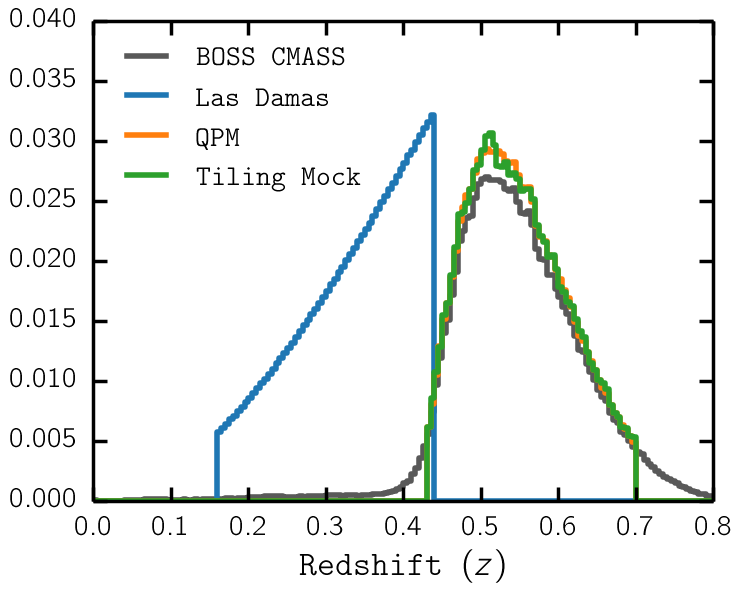
\includegraphics[scale=0.45]{fcpaper_z_dist.png} \label{fig:zdist}
\caption{Normalized galaxy redshift distribution for Las Damas (\ldgcolor), QPM (\qpmcolor), and Tiling Mock (\tmcolor) mock catalogues. The normalized redshift distribution of BOSS DR12 CMASS is also plotted (\cmasscolor). Bin size of $\Delta z = 0.025$ was used to compute the distributions. Las Damas mock catalogue has a constant number density of galaxies throughout its redshift range ($0.16 < z < 0.44$). QPM and Tiling Mock catalogues, on the other hand, trace the BOSS CMASS redshift distribution ($0.43 < z < 0.7$).}
% perhaps the range should be wider and make it full text width that way the tail can be portrayed better. Keep the same aspect ratio. 
\end{center}
\end{figure}

Effects of fiber-collisions must be understood and interpreted in conjunction with these systematic effects and to ultimately test our fiber-collision correction method we use LasDamas (\citealt{McBride:2009aa}), Quick Particle Mesh (\citealt{White:2014aa}), and Tiling mock catalogues. These mocks have already been used in interpreting observational results for BOSS and are generated through different prescriptions. Therefore they provide complementary tests fiber-collisions and our correction method tailored for BOSS. 
% Include brief detail on what each mock has to offer

Each of these mock catalogues use some sort of N-body dark matter simulation along with a HOD prescription to populate the dark matter halos with ``galaxies". More specifically, the LasDamas Galaxy mock catalogues is constructed from the N-body Large Suite of Dark Matter Simulations (LasDamas). The N-body LasDamas simulations uses a spatially flat $\Lambda$CDM cosmology with $\Omega_\mathrm{m} = 0.25$, $\Omega_\Lambda = 0.75$, $\Omega_\mathrm{b} = 0.04$, $\sigma_8 = 0.8$, $n_\mathrm{s} = 1$ and $h=0.7$. The dark matter halos are then identified using a friends-of-friends (FOF) algorithm (\citealt{Davis:1985aa}) with a linking length $b = 0.2 $ times the mean interparticle separation. The over-densities of dark matter halos are then populated with galaxies using the halo occupation distribution (HOD) framework to construct the galaxy mock catalogues (\citealt{McBride:2009aa}). The HOD prescription is specified so that the galaxy mock catalogues reproduce the correlation function of the SDSS sample. % Detail about the geometry and redshift range 
\begin{itemize}
\item above description is not entirely correct because that was LasDamas for Guo+2011
\item SDSS-II Geometry
\item lower redshift range
\end{itemize}

Next, the QPM mock galaxy catalogues uses a "quick particle mesh" method, which uses a low resolution particle-mesh N-body solver to evolve particles within a period simulation volume. The particles are assigned halo masses  in order to match the halo mass function and large-scale bias of halos of high resolution simulations. Afterward the \cite{Tinker:2012aa} HOD parameterization is used to populate the halos. The mock galaxy sample is then trimmed to the BOSS CMASS survey footprint, downsamped based on angular sky completeness (sector completeness) and radial selection. The QPM mock galaxy catalogue is generated using the following $\Lambda$CDM cosmology: $\Omega_\mathrm{m} = 0.25$, $\Omega_\Lambda = 0.25$, $\Omega_\mathrm{b} = 0.04$, $\sigma_8 = 0.8$, $n_\mathrm{s} = 1$ and $h=0.7$. For a detailed description of the QPM galaxy mock catalogues we refer readers to \cite{White:2014aa}. 

Finally the Tiling Mock catalogue is generated using 
\begin{itemize}
\item documentation for tiling mock? 
\end{itemize}

In Figure \ref{fig:zdist}, we plot the redshift distribution for LasDamas, QPM, and Tiling Mock catalogues along with the redshift distribution of BOSS DR12 galaxies. The redshift distributions illustrate the constant $\bar{n}(z)$ for the LasDamas mock catalogue, while the QPM and Tiling mock $\bar{n}(z)$ distributions trace the observed BOSS redshift distribution. 

% insert transition that mentions how the main clustering statistics we focus on in this paper is the Power Spectrum
In order to measure the power spectrum for these mock catalogues, we use the standard \cite{Feldman:1994aa} (FKP) estimator. Throughout the paper we use the following formalisms from \cite{Feldman:1994aa}.
\begin{equation} \label{eq:fkppk}
P({\bf k}) = <|F({\bf k})|^2> - \frac{(1+\alpha) \int d^3r \;\bar{n}({\bf r})w_{\mathrm{FKP}}^2({\bf r})} {\int d^3r \; \bar{n}^2({\bf r})w_{\mathrm{FKP}}^2({\bf r})},
\end{equation}  
where
\begin{equation}
F({\bf r}) = \frac{w_\mathrm{FKP}({\bf r}) [n_g({\bf r}) - \alpha n_r({\bf r})]} {[\int d^3r \; \bar{n}^2({\bf r})w_\mathrm{FKP}^2({\bf r})]^{\frac{1}{2}}} 
\end{equation}
and the second term represents the constant shot-noise contribution to the power due to the discrete density field of our galaxies. More specifically, $n_g$ is the galaxy density, $n_r$ is the density of the synthetic random catalogue, $\alpha$ is the ratio of the number of galaxies over the number of synthetic random galaxies, $\bar{n}$ is the mean density of the galaxies, and $w_{\mathrm{FKP}}$ is the minimum variance weight derived in \cite{Feldman:1994aa}: 
\begin{equation}
w_{\mathrm{FKP}} ({\bf r}) = \frac{1}{1+\bar{n}({\bf r}) P_0}
\end{equation}
where $P_0$ is the power spectrum amplitude at which the error is minimized. We use $P_0 = 20000\; \mathrm{Mpc}^3/h^3$ for our analysis, which corresponds to $k \sim 0.1\; h/\mathrm{Mpc}$.  

\begin{figure}
\begin{center}
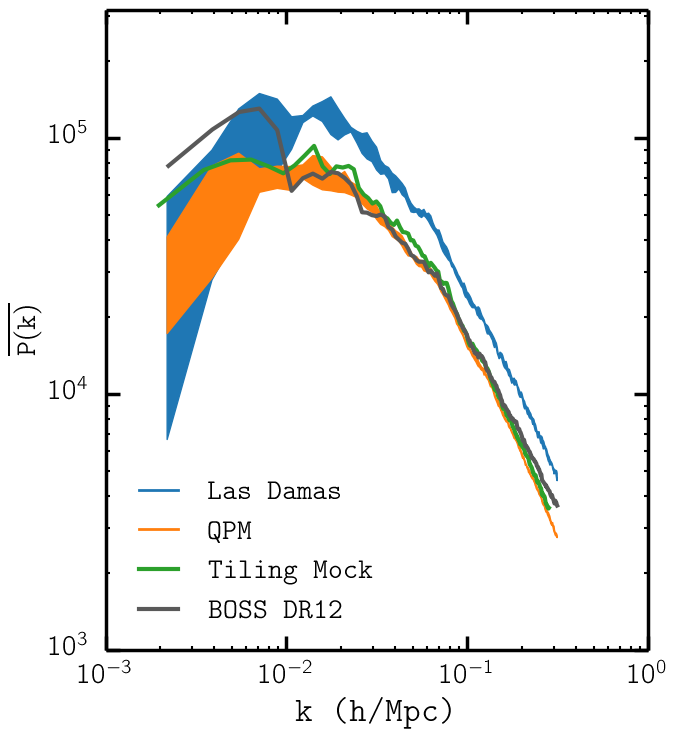
\includegraphics[scale=0.5]{fcpaper_pk_comp.png} 
\caption{Average power spectrum $\overline{P(k)}$ for BOSS DR12 (black) and the mock catalogues Las Damas (blue), QPM (orange), and Tiling Mock (green), listed in Section \ref{sec:catalog} using the FKP $P(k)$ estimator. The width of the $P(k)$ for Las Damas and QPM represent the sample variance ($\Delta P(k)/\overline{P(k)}$) calculated from the multiple mock catalogues. We emphasize that fiber-collisions were not applied to the mock catalogues for the $P(k)$ measurements. Meanwhile, galaxy weights (Equation \ref{eq:weight}) are applied to the BOSS DR12 $P(k)$ measurement. We remind readers that the $\overline{P(k)}$ of the LasDamas mock catalogues is an outlier because of the different redshift range compared to the other mock catalogues.} \label{fig:mockpk}
\end{center}
\end{figure}

For LasDamas, QPM, and Tiling mock catalogues we use the above FKP estimator to measure the power spectrum, Figure \ref{fig:mockpk}. For the $P(k)$ in Figure \ref{fig:mockpk}, we do not apply the fiber-collisions to the catalogues. Therefore, there are no complications from using the exact formulation of Equation \ref{eq:fkppk}. However, when we calculate $P(k)$ for BOSS DR12 data in Figure \ref{fig:mockpk} (\cmasscolor), the systematic weights assigned to the galaxies that account for sector completeness, redshift failures, and fiber-collisions, 
\begin{equation} \label{eq:weight}
w_\mathrm{tot} = w_\mathrm{sys} (w_\mathrm{rf} + w_\mathrm{fc} -1), 
\end{equation}
must be taken account (\citealt{Anderson:2012aa, Beutler:2014aa}). Hence, instead of the galaxy density $n_g({\bf r})$ we use a weighted galaxy density $n'_g({\bf r}) = n_g({\bf r}) w({\bf r})$ and instead of $\alpha = N_{\mathrm{gal}}/N_\mathrm{ran}$ we use $\alpha ' = N'_\mathrm{gal}/N_\mathrm{ran}$ where $N'_\mathrm{gal} = \sum_\mathrm{gal} w_\mathrm{tot}$. For LasDamas and QPM, which have multiple mock catalogues, we compute the sample variance of the power spectrum
\begin{equation} \label{eq:pk_var}
\Delta P (k)= \sqrt{\frac{1}{N_\mathrm{mock}} \sum\limits_i^{N_\mathrm{mock}} (P_i(k)- \overline{P(k)})^2 }. 
\end{equation}
$\Delta P(k)$ is represented by the width of the $P(k)$ in Figure \ref{fig:mockpk}. 

\begin{figure*}
\begin{center}
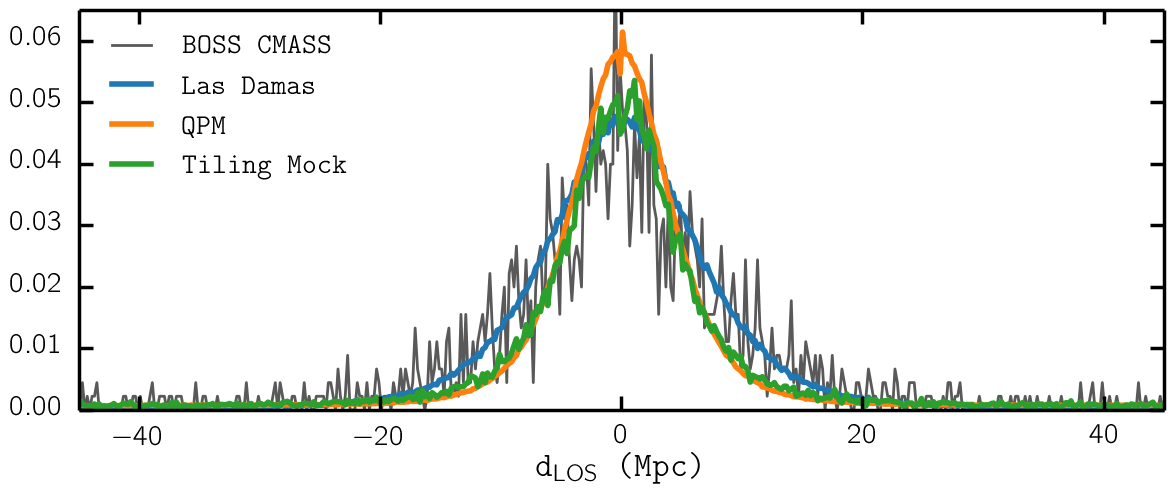
\includegraphics[scale=0.575]{fcpaper_dlos_dist.png}
\caption{Normalized distribution of $d_{\mathrm{LOS}}$ for Las Damas (\ldgcolor), QPM (\qpmcolor), and Tiling Mock (\tmcolor) mock catalogues. The normalized $d_{\mathrm{LOS}}$ distribution of BOSS DR12 is also plotted (\cmasscolor). Bin size of $\Delta d = 0.2$ was used to compute these $d_{\mathrm{LOS}}$ distributions. We focus on the peak of the distribution (discussed in \ref{sec:dlos}).} \label{fig:d_los}
% perhaps the range should be wider and make it full text width that way the tail can be portrayed better. Keep the same aspect ratio. 
\end{center}
\end{figure*}

%%%%%%%%%%%%%%%%%%%%%%%%%%%%%%%%%%%%%%%%%%%%%%%%%%%%%%%%%%%%%%%%%%%%%%%%%%%%%%
% Fiber-collision Correction Method
%%%%%%%%%%%%%%%%%%%%%%%%%%%%%%%%%%%%%%%%%%%%%%%%%%%%%%%%%%%%%%%%%%%%%%%%%%%%%%
\section{Fiber-collision Correction Method} \label{sec:fc_corr}
To account for the systematic effects of fiber-collisions \cite{Anderson:2012aa}, for the BOSS galaxy data, most recently used a nearest-neighbor galaxy weighting scheme. For galaxies without resolved spectroscopic redshifts due to fiber-collisions, the entire statistical weight of the galaxy was assigned to its nearest-neighbor. This method assumes that all galaxies with angular separations $< 62 "$ are correlated. In other words, that galaxies within the fiber-collision angular scale reside in the same group or cluster. Consequently, galaxies that have angular separations $< 62"$ purely by coincidence (hereafter referred to as ``chance alignments") are incorrectly assumed to be gravitationally correlated and displaced significantly from its true position. Even for fiber-collided galaxies that reside in the same group or cluster, upweighting the nearest neighbor ignores halo-scale line-of-sight displacements. 

While the nearest-neighbor method provides a reasonable estimate at large scales, in Section \ref{sec:dlos} we demonstrate that at small scales it's effects on the power spectrum are significant and outweigh sample variance. Furthermore, in Section \ref{sec:dlos}, we present an improved method to account for correlated fiber-collided galaxies using the line-of-sight displacement between close galaxy pairs. Then in Section \ref{sec:shotnoise}, we present corrections to the power spectrum estimator that further accounts for fiber-collisions through the shot-noise correction term in the estimator. 

%%%%%%%%%%%%%%%%%%%%%%%%%%%%%%%%%%%%%%%%%%%%%%%%%%%%%%%%%%%%%%%%%%%%%%%%%%%%%%
% LOS DISPLACEMENT
%%%%%%%%%%%%%%%%%%%%%%%%%%%%%%%%%%%%%%%%%%%%%%%%%%%%%%%%%%%%%%%%%%%%%%%%%%%%%%
\subsection{Line-of-Sight Displacement of Fiber-collided Pairs} \label{sec:dlos}
It is impossible to determine in observed galaxy data whether fiber-collided galaxies without resolved spectroscopic redshift are either correlated or chance alignments. Fortunately, using just the close galaxy pairs with resolved redshifts (especially in the overlapping regions mentioned in Section \ref{sec:catalog}), it is possible to model the fraction of galaxy pairs that are corrected and uncorrelated. 

Meanwhile, for simulated mock catalogues, described in Section \ref{sec:catalog}, modeling the fiber-collided galaxy pairs is a trivial task since fiber-collisions are post-processed after the simulated galaxy positions are generated. Hence all redshift values are resolved regardless of angular proximity. With both redshifts of the fiber-collided pair galaxies, we are able to emulate the observed data by assigning nearest neighbor galaxy weights (as done in \citealt{Anderson:2012aa}). So for a close galaxy pair, one galaxy (``the nearest neighbor") will have the statistical weight of both galaxies, while the other has a statistical weight of $0$. Furthermore, having the redshift values of close galaxy pairs in mock catalogues, allows us to model the correlated and uncorrelated fiber-collided pairs. 

In order to determine whether or not fiber-collided pairs are correlated, we examine the comoving line-of-sight displacement ($d_{\mathrm{LOS}}$) of fiber-collided galaxy pairs. We calculate the $d_{\mathrm{LOS}}$ by taking the difference of the line-of-sight comoving distance from the resolved redshifts: 
\begin{equation}
d_{\mathrm{LOS}} = D_{\mathrm{C}} (z_1) - D_{\mathrm{C}} (z_2). 
\end{equation}
$D_{\mathrm{C}}(z)$ is the line-of-sight comoving distance at redshift $z$ (\citealt{Hogg:1999aa}). $z_1$ and $z_2$ represent the resolved redshifts of the galaxies in the fiber-collided pair.

After calculating the $d_{\mathrm{LOS}}$ for each of the fiber-collided pairs, in Figure \ref{fig:d_los} we present the distribution of $d_{\mathrm{LOS}}$ for LasDamas (\ldgcolor), QPM (\qpmcolor), Tiling Mock (\tmcolor), and BOSS DR12 (\cmasscolor). All of the $d_{\mathrm{LOS}}$ distributions contain two distinct components: a peak approximately within the range $-10\;\mathrm{Mpc} < d_{\mathrm{LOS}} < 10\;\mathrm{Mpc}$ and a flat component (hereafter "tail" component) that extends to $d_{\mathrm{LOS}}$ that encompasses the survey depth (entire range of the distribution not displayed in Figure \ref{fig:d_los}). We note that for the BOSS data, since we cannot compute the $d_\mathrm{LOS}$ for fiber-collided pairs without resolved spectra, the $d_\mathrm{LOS}$ distribution represents the $d_\mathrm{LOS}$ from close galaxy pairs with resolved spectroscopic redshifts, often from overlapping regions of the BOSS survey.

Galaxies that are in the same groups or clusters, due to their gravitational interactions at halo-scales, are more likely to be in close angular proximity with each other. These galaxies in over-dense regions cause the peak in the $d_{\mathrm{LOS}}$ distribution. While the ``tail" component is composed of galaxy pairs that are arbitrarily in close angular proximity even when they are not correlated. 

Focusing on the peak of the distribution, we note that it closely traces an exponential function. Therefore, we fit an exponential of the form, 
\begin{equation} \label{eq:peak} 
p(d_{\mathrm{LOS}}) = A \; e^{-|d_{\mathrm{LOS}}|/\sigma}
\end{equation}
 for a mathematical prescription of the $d_{\mathrm{LOS}}$ distribution peak as a function of the displacement for each of the data catalogues in Figure \ref{fig:d_los}. The best-fit $\sigma$ and $A$ parameters are obtained by fitting Equation \ref{eq:peak} to the $d_{\mathrm{LOS}}$ distribution peaks using MPFIT (\citealt{Markwardt:2009aa}). We list the values of $\sigma$ obtained for the mock catalogues in Table \ref{tab:mpfit}. Both Table \ref{tab:mpfit} and Figure \ref{fig:d_los} illustrate that the $d_{\mathrm{LOS}}$ distributions for the mock catalogues closely trace the distribution of the BOSS DR12, which further goes to support our use of mock catalogues to test our fiber-collision correction method. 
 
 \begin{table} 
 \caption{$d_{\mathrm{LOS}}$ Distribution Best-fit Parameters} \label{tab:mpfit}
 \begin{spacing}{1.5}
 \begin{center}
 \leavevmode
 \begin{tabular}{ccc} \hline \hline
Catalogue &$\sigma$ ($h^{-1}\mathrm{Mpc}$) & $f_{\mathrm{peak}}$\\ \hline
Las Damas 	& 6.85	& 0.71 \\ 
QPM 		& 4.98	& 0.65 \\ 
Tiling Mock 	& 5.38	& 0.57 \\ 
BOSS DR12 	& 7.6		& 0.65 \\ \hline
\end{tabular} \par
\end{center}
\end{spacing}
%    \bigskip 
{\bf Notes}: Best-fit parameter $\sigma$ and peak fraction $f_{\mathrm{peak}}$ for the $d_{\mathrm{LOS}}$ distributions in Figure \ref{fig:d_los}. 
\end{table}

Using the exponential fits to the peak of the $d_{\mathrm{LOS}}$ distribution, we can also estimate the fraction of fiber-collided pairs that are within the peak: 
\begin{equation}
f_{\mathrm{peak}} = \frac{\sum\limits_{\mathrm{peak}} p(d_{\mathrm{LOS}})}{N_{\mathrm{pairs}}}, 
\end{equation}
where $N_{\mathrm{pairs}}$ is the total number of fiber-collided pairs. As mentioned above, this portion of fiber-collided pairs are galaxy pairs that are correlated. We list the $f_{\mathrm{peak}}$ values for each of the data catalogues in Table \ref{tab:mpfit}. The $f_\mathrm{peak}$ values for the mock catalogue are also in good agreement with the BOSS DR12 $f_\mathrm{peak}$. 

As stated earlier, the current method of accounting for fiber-collisions uses the nearest-neighbor upweighting scheme (hereafter NN-upweighting). For this method to be completely correct, the $d_{\mathrm{LOS}}$ distribution would have to be a delta function, which as Figure \ref{fig:d_los} demonstrates is not the case. By simply incorporating the peak of the $d_{\mathrm{LOS}}$ distribution, we are able to significantly improve clustering statistics on small scales. Rather than placing the fiber-collided galaxy on top of its nearest neighbor, as NN-upweighting does, placing the fiber-collided galaxy at displacement sampled from the $d_{\mathrm{LOS}}$ distribution, away from the nearest neighbor better accounts for the small scale clustering measurements. On mock catalogues, we test this by first applying the NN upweighting in the same way as it is applied in the BOSS DR12 catalogue to the mock catalogues. We then sample a displacement $d_i$ from $p(d_\mathrm{LOS})$ (Equation \ref{eq:peak}) for each fiber-collided pair. Afterwards we ``place" the fiber-collided galaxy a distance $d_i$ from the upweighted galaxy and reduce the statistical weight of the upweighted galaxy (the nearest-neighbor) by 1. We refer to this method as ``$d_\mathrm{LOS}$-peak. 

\begin{figure*}
\begin{center}
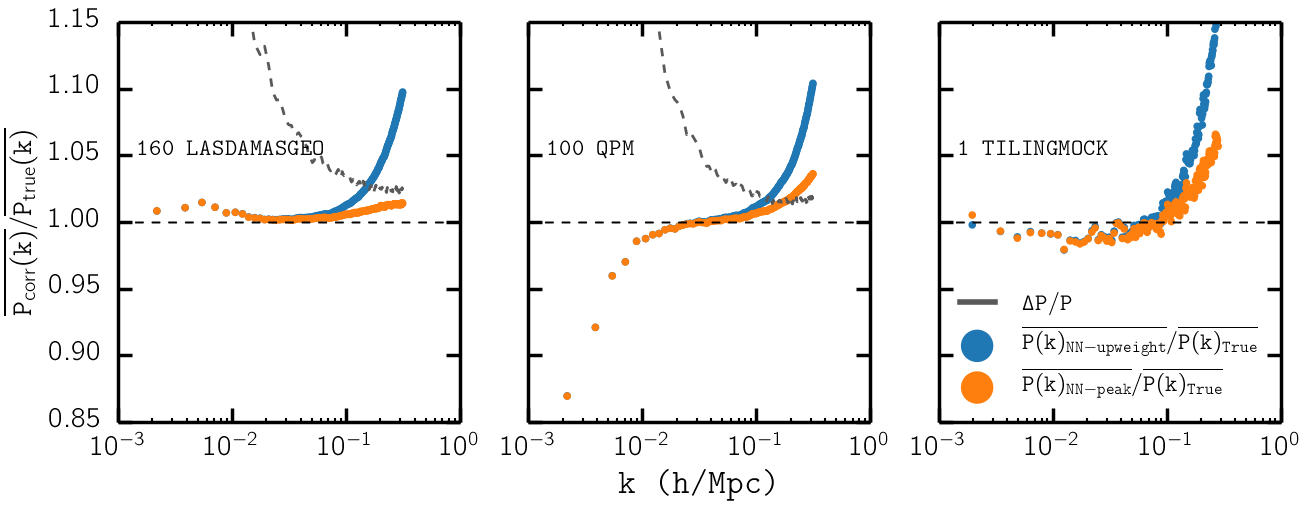
\includegraphics[scale=0.55]{fcpaper_pk_peakonly_comp.png} 
\caption{The ratio of $P(k)$ using the nearest-neighbor upweighting (blue) and $d_\mathrm{LOS}$ distribution peak fiber-collision correction (orange) over the true $P(k)$ for LasDamas (left panel), QPM (middle panel), and Tiling Mock (right panel) catalogues. }\label{fig:peakonly}
\end{center}
\end{figure*}

The $d_\mathrm{LOS}$-peak correction method is only part of our correction scheme we present in this paper. Nonetheless, we test it by applying it to the mock catalogues and comparing the resulting power spectrums. For each of the mock catalogues (Las Damas, QPM, and Tiling Mock) we use the FKP power spectrum estimator from before to compute the power spectrums of the original mock data, the mock data with NN-upweighting, and the mock data with the $d_\mathrm{LOS}$-peak correction. We note that both the NN-upweighting and the $d_\mathrm{LOS}$-peak correction methods alter the redshift distribution of our samples by a negligible amount $< 1\%$. Therefore, the synthetic random catalogues and the $\bar{n}(z)$ values do not need to be adjusted in the FKP $P(k)$ calculations.

Since we are interested in how well these fiber-collision considerations can reproduce the power spectrum without fiber collisions (the ``true" power spectrum, unsullied by systematic effects), in Figure \ref{fig:peakonly} we plot the ratio of the average power spectrum $P(k)$ computed from corrected mock catalogues over the average $P(k)$ from the original mock catalogues, $\overline{P_{\mathrm{corr}}(k)}/\overline{P_\mathrm{true}(k)}$. The ratio for the NN upweighting scheme is plotted in blue while the ratio for the $d_{\mathrm{LOS}}$-peak correction scheme is plotted in orange. Also plotted is $\Delta P_\mathrm{true}(k) / \overline{P_\mathrm{true}(k)}$ (black; dashed) in order to compare the ratios to sample variance of the mock catalogues. For all mocks, the $P(k)$ from the NN upweighting scheme is greater than $P_\mathrm{true}(k)$ by $> 10 \%$ at $ k \sim 0.3\; h/\mathrm{Mpc}$. In comparison, $P(k)$ from the $d_\mathrm{LOS}$-peak correction method is $\sim 5\%$ greater than $P_\mathrm{true}(k)$ - a significant improvement. 

Comparing the NN-upweighting and the $d_\mathrm{LOS}$-peak methods to the sample variance ($\Delta P_\mathrm{true}(k) / \overline{P_\mathrm{true}(k)}$), reveal that neither of these methods provide a sufficient correction for the fiber-collision at $k > 0.1\; h/\mathrm{Mpc}$. The $P(k)$s obtained from these methods are dominated by systematics on small scales. Furthermore, the $d_\mathrm{LOS}$-peak method only statistically accounts for correlated pairs and does not consider uncorrelated pairs. Using the entire $d_\mathrm{LOS}$ distribution in order to account for uncorrelated pairs results in an overall reduction of $P(k)$ since the method displaces some close pairs that are actually correlated pairs as uncorrelated pairs and the other way around. Therefore, a more robust fiber-collision correction method is required. 
%detailed examination of peak only figure 

\begin{figure*}
\begin{center}
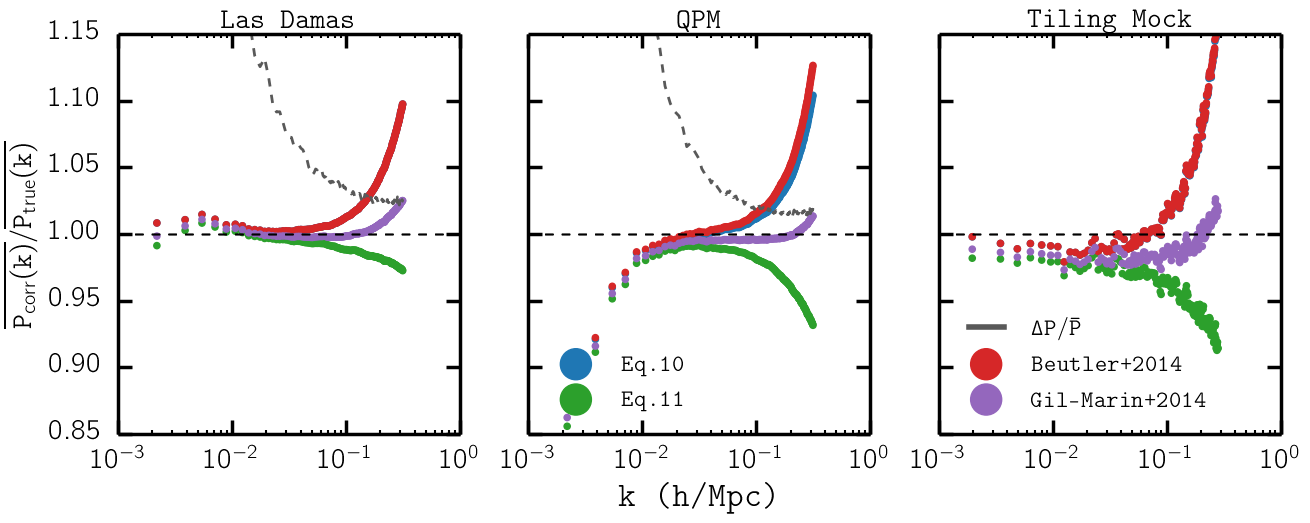
\includegraphics[scale=0.55]{fcpaper_pk_shotnoiseonly_comp.png}
\caption{The ratio of $\overline{P_\mathrm{SN}(k)}$ computed using the shot-noise correction term given by Eq. \ref{eq:fkp_shotnoise} (blue), Eq. \ref{eq:my_shotnoise} (green), $P^\mathrm{Beutler}_\mathrm{shot}$ (red), and $P^{\mathrm{Gil-Marin}}_\mathrm{shot}$ (purple) over $\overline{P_\mathrm{true}(k)}$ for LasDamas (left panel), QPM (middle panel), and Tiling Mock (right panel) catalogues with nearest-neighbor fiber-collision weights. Also plotted for comparison, is $\Delta P_\mathrm{true}/P_\mathrm{true}(k)$. For fiber-collisions  $\overline{P_\mathrm{SN}(k)}$ computed using $P^\mathrm{Beutler}_\mathrm{shot}$ only marginally improves the $\overline{P_\mathrm{SN}(k)}$ computed using $P^\mathrm{FKP}_\mathrm{shot}$. Both $\overline{P_\mathrm{SN}(k)}$s significantly overestimates the power spectrum. On the other hand $\overline{P_\mathrm{SN}(k)}$ computed using Eq. \ref{eq:my_shotnoise} significantly underestimates the power spectrum. At $k \sim 0.3\;h/\mathrm{Mpc}$, only $\overline{P_\mathrm{SN}(k)}$ computed using $P^\mathrm{Gil-Marin}_\mathrm{shot}$ reduces the effect of fiber-collisions below sample variance. } \label{fig:shotnoise}
\end{center}
\end{figure*}
%%%%%%%%%%%%%%%%%%%%%%%%%%%%%%%%%%%%%%%%%%%%%%%%%%%%%%%%%%%%%%%%%%%%%%%%%%%%%%
% SHOT NOISE CORRECTION 
%%%%%%%%%%%%%%%%%%%%%%%%%%%%%%%%%%%%%%%%%%%%%%%%%%%%%%%%%%%%%%%%%%%%%%%%%%%%%%
\subsection{Shot Noise Correction} \label{sec:shotnoise} 
Both the NN-upweighting and the $d_\mathrm{LOS}$-peak correction schemes do not sufficiently account for the systematic effects of fiber-collisions in the power spectrum. In this section we introduce the other part of our fiber-collision correction method that involve the shot-noise correction term of the power spectrum estimator. 
%Besides illustrating the short comings of the NN-upweighting scheme and also the $d_\mathrm{LOS}$ distribution peak correction scheme, in Section \ref{sec:dlos}, we briefly mentioned that the \cite{Feldman:1994aa} power spectrum estimator was used to compute the power spectrum.  % possibly insert summary of the actual power spectrum estimator calculation

In Section \ref{sec:catalog}, we described the FKP power spectrum estimator used to compute the power spectrums of Figure \ref{fig:mockpk}. In their estimator, to account for the discreteness of the density field, they subtract the shot-noise contribution to the power spectrum (Equation \ref{eq:fkppk}): 
\begin{equation} \label{eq:fkp_shotnoise}
P_\mathrm{shot} = \frac{ (1+\alpha) \int d^3r \;\bar{n}({\bf r})w^2({\bf r})}{\int d^3r \;\bar{n}^2({\bf r})w^2({\bf r})}. 
\end{equation}
In practice, the integrals in Equation \ref{eq:fkp_shotnoise} can be written in terms of discrete sums over the random catalogue. The spacial integral $\int d^3r \; \bar{n}({\bf r}) ...$ can be computed as the discrete sum $\alpha \sum_{\mathrm{ran}}...$. With this conversion,
\begin{equation}
P^\mathrm{FKP}_\mathrm{shot} = \frac{(1+\alpha) \alpha \sum\limits_{\mathrm{random}} w_\mathrm{FKP}^2({\bf r})}{\alpha \sum\limits_{\mathrm{random}}w_\mathrm{FKP}^2({\bf r})}.
\end{equation} 
In the FKP derivation, they do not take systematic weights of galaxies into account.

The spatial integral $\int d^3r \;\bar{n}({\bf r})...$ can also be computed using the mock catalogues rather than the synthetic random catalogues, as $\sum_{\mathrm{gal}} w_g...$ where $w_g$ represents the statistical weight assigned to the galaxies (\citealt{Cole:2005aa, Yamamoto:2006aa, Beutler:2014aa, Gil-Marin:2014aa}). Then the shot-noise component can be expressed as: 
\begin{equation} \label{eq:fkpweight}
P_\mathrm{shot} = \frac{ \sum\limits_{\mathrm{galaxy}} w^2_\mathrm{FKP}w^2_g({\bf r})- \alpha^2 \sum\limits_{\mathrm{random}} w_\mathrm{FKP}^2({\bf r})}{\alpha \sum\limits_{\mathrm{random}}w_\mathrm{FKP}^2({\bf r})}.
\end{equation}
In this form, systematic weights for galaxies can be accounted for in $w_g$ and $\alpha$. 

Following the latter formulation, most recently, both \cite{Beutler:2014aa} and \cite{Gil-Marin:2014aa} formulate $P_\mathrm{shot}$ to account for systematic bias in their analysis of BOSS data. However, they treat systematic weights differently in their derivation. Keeping in mind the weights listed in Eq. \ref{eq:weight} for the BOSS data, \cite{Beutler:2014aa} derives
\begin{equation} \label{eq:florian}
P^\mathrm{Beutler}_\mathrm{shot} = \frac{\sum\limits_{\mathrm{galaxy}} w^2_\mathrm{FKP}w_\mathrm{tot}({\bf r})w_\mathrm{sys}({\bf r}) - \alpha'^2 \sum\limits_{\mathrm{random}} w_\mathrm{FKP}^2({\bf r})}{\alpha' \sum\limits_{\mathrm{random}}w_\mathrm{FKP}^2({\bf r})}.
\end{equation}
$\alpha' = \sum_\mathrm{gal} w_\mathrm{tot} / N_\mathrm{ran}$. 

On the other hand, \cite{Gil-Marin:2014aa}, in a formulation designed to account for fiber-collisions derives $P_\mathrm{shot}$ using two separate components: one for correlated pairs and the other chance alignments. For the shot-noise contribution to the power from correlated pairs (referred to as ``true pairs" in \citealt{Gil-Marin:2014aa}) is equivalent to $P^\mathrm{Beu2tler}_\mathrm{shot}$ in \cite{Beutler:2014aa}. For chance alignments (referred to as ``false pairs" in \citealt{Gil-Marin:2014aa}), the shot-noise contribution is derived as, 
\begin{equation}
P^\mathrm{False}_\mathrm{shot} = \frac{\sum\limits_{\mathrm{galaxy}} w^2_\mathrm{FKP}w^2_\mathrm{tot}({\bf r}) - \alpha'^2 \sum\limits_{\mathrm{random}} w_\mathrm{FKP}^2({\bf r})}{\alpha' \sum\limits_{\mathrm{random}}w_\mathrm{FKP}^2({\bf r})}.
\end{equation}
Then the total $P_\mathrm{shot}$ is calculated as a combination of $P^\mathrm{True}_\mathrm{shot}$ and $P^\mathrm{False}_\mathrm{shot}$: 
\begin{equation}
P^\mathrm{Gil-Marin}_\mathrm{shot} = (1- x_\mathrm{PS}) P^{True}_\mathrm{shot} + x_\mathrm{PS} P^{False}_\mathrm{shot}
\end{equation}
For the BOSS $P(k)$ \cite{Gil-Marin:2014aa} quotes $x_\mathrm{PS} = 0.58$. %motivation for the true/false pairs? 

In our $P(k)$ calculations we use the FKP estimator with the shot-noise correction term computed as Eq. \ref{eq:fkpweight} with $w_\mathrm{g} = w_\mathrm{tot}$, which gives us, 
\begin{equation} \label{eq:ourshot}
P^\mathrm{Hahn\;et\;al.}_\mathrm{shot} = \frac{\sum\limits_{\mathrm{galaxy}} w^2_\mathrm{FKP}w^2_\mathrm{tot}({\bf r}) - \alpha'^2 \sum\limits_{\mathrm{random}} w_\mathrm{FKP}^2({\bf r})}{\alpha' \sum\limits_{\mathrm{random}}w_\mathrm{FKP}^2({\bf r})}.
\end{equation}
We note that this equation is equivalent to the shot-noise contribution from ``false pairs" in \cite{Gil-Marin:2014aa}. 
%In \cite{Gil-Marin:2014aa}, they justify the use of the two separate shot-noise terms with the argument that, if the fiber-collided pairs are true pairs it would not modify %insert reason 
%While the $P(k)$ using the \cite{Gil-Marin:2014aa} shot-noise term does in fact correct for fiber-collisions significantly (below), since the parameter is determined in mock catalogues, the value cannot be validated in the actual BOSS data .

In order to compare the different $P_\mathrm{shot}$ derivations, we apply each of them ($P^\mathrm{FKP}_\mathrm{shot}$,$P^\mathrm{Hahn}_\mathrm{shot}$, $P^\mathrm{Beutler}_\mathrm{shot}$, and $P^\mathrm{Gil-Marin}_\mathrm{shot}$) to the mock catalogues with nearest-neighbor fiber-collision weights applied to them. This comparison ignores a number of systematic effects listed in Eq. \ref{eq:weight} ($w_\mathrm{sys}$ and $w_\mathrm{rf}$); however, we are particularly interested in fiber-collisions. So in Equations 9-15, we use $w_\mathrm{sys} = 1$ and $w_\mathrm{tot} = w_\mathrm{fc}$. We compute the $P_\mathrm{SN}(k)$s using the various $P(k)$ estimators with different $P_\mathrm{shot}$ equations for each of the mock catalogues. Afterwards we compute the $\overline{P_\mathrm{SN}(k)}$s for the mock catalogues and take the ratio of them over the average $P_\mathrm{true}(k)$ using the standard FKP $P(k)$ estimator. Without systematic weights, the different $P_\mathrm{shot}$ equations are equivalent, so our choice of the standard FKP $P(k)$ estimator for $\overline{P_\mathrm{true}(k)}$ does not affect the comparison. 

In Figure \ref{fig:shotnoise}, we present $\overline{P_\mathrm{SN}(k)}/\overline{P_\mathrm{true}(k)}$ computed using different shot noise correction term equations: $P^\mathrm{FKP}_\mathrm{shot}$,$P^\mathrm{Hahn}_\mathrm{shot}$, $P^\mathrm{Beutler}_\mathrm{shot}$, and $P^\mathrm{Gil-Marin}_\mathrm{shot}$. The $\overline{P(k)}$ of the NN-upweighted mocks using the standard FKP estimator is the same quantity as presented in Figure \ref{fig:peakonly} and as we noted earlier, overestimates the $\overline{P_\mathrm{true}(k)}$. $\overline{P_\mathrm{FKP}(k)}$ is greater than $\overline{P_\mathrm{true}(k)}$ by $> 15 \%$ at $k \sim 0.3\; h/\mathrm{Mpc}$. The $\overline{P(k)}$ measured using $P^\mathrm{Beutler}_\mathrm{shot}$ does not improve this overestimation in any of the mocks. On the other hand, the $\overline{P(k)}$ using just our shot noise equation significantly underestimates the $\overline{P_\mathrm{true}(k)}$. At $k \sim 0.3 \; h/\mathrm{Mpc}$, $\overline{P(k)}/\overline{P_\mathrm{true}(k)} - 1 = \sim -0.03 \%, \sim -0.08 \%, \;\mathrm{and} \sim -0.09$ for LasDamas, QPM, and Tiling Mock respectively. Finally, the $\overline{P(k)}$ measured using $P^\mathrm{Gil-Marin}_\mathrm{shot}$ reproduces $\overline{P_\mathrm{true}(k)}$ most accurately. % Insert some more specifics about Hector's accuracy

As we plotted in Figure \ref{fig:peakonly}, we plot the sample variance ($\Delta P/\bar{P}$) for each of the mock catalogues in Figure \ref{fig:shotnoise}. Only $\overline{P(k)}$ computed using $P^\mathrm{Gil-Marin}_\mathrm{shot}$ is able to reduce the effects of fiber-collisions below the sample variance. 

With these alterations to the power spectrum estimator in mind, we present our fiber-collision correction method in the following section . 

%%%%%%%%%%%%%%%%%%%%%%%%%%%%%%%%%%%%%%%%%%%%%%%%%%%%%%%%%%%%%%%%%%%%%%%%%%%%%%%%
% RESULT
%%%%%%%%%%%%%%%%%%%%%%%%%%%%%%%%%%%%%%%%%%%%%%%%%%%%%%%%%%%%%%%%%%%%%%%%%%%%%%%%
\section{Results} 
\subsection{Fiber-Collision Correction Method} \label{sec:apply} 
\begin{figure*}
\begin{center}
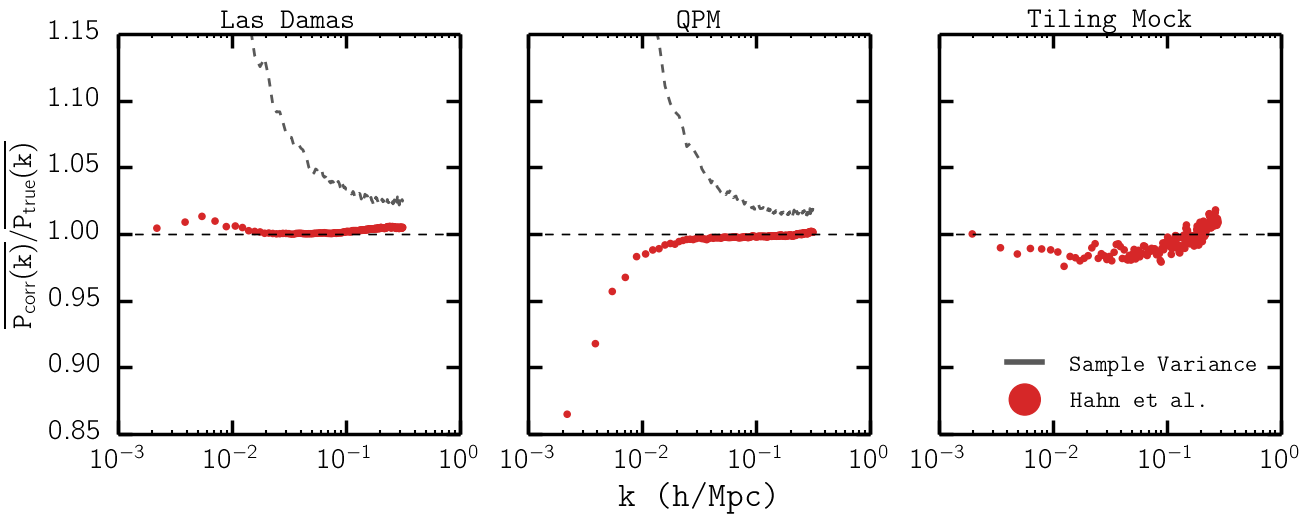
\includegraphics[scale=0.55]{fcpaper_pk_peakshotnoise_mpfit_comp.png} 
\caption{The ratio of $\overline{P(k)}$ computed using our fiber-collision correction method described in Section \ref{sec:apply} over $\overline{P_\mathrm{true}(k)}$ for LasDamas (left panel), QPM (middle panel), and Tiling Mock (right panel) catalogues with nearest-neighbor fiber-collision weights (red). Also plotted for comparison, is $\Delta P_\mathrm{true}/P_\mathrm{true}(k)$. We note that the $\overline{P(k)}$ ratio for our correction method is significantly lower than the $\Delta P_\mathrm{true}/P_\mathrm{true}(k)$.}\label{fig:peaksn}
\end{center}
\end{figure*}

In Section \ref{sec:dlos} we derive a method to account for fiber-collisions using the peak of the $d_\mathrm{LOS}$ distribution. Then in Section \ref{sec:shotnoise} we compare the various formulations for the shot-noise correction term and presented our formulation. We now utilize both methods to devise our fiber-collision correction method. 

We begin with the nearest-neighbor upweighted mock catalogues. With the nearest-neighbor fiber-collision weights, these mock catalogues accurately imitate the effects of fiber-collision on the real BOSS data. Then as described in Section \ref{sec:dlos}, we calculate the $d_\mathrm{LOS}$ distribution of all fiber-collided pairs in each mock catalogue. Using the $d_\mathrm{LOS}$ distribution, we compute the fraction of close pairs that are contained within the peak of the distribution ($f_\mathrm{peak}$; Section \ref{sec:dlos}). We then select $f_\mathrm{peak}$ of the close pairs and treat them as correlated pairs that lie in the peak of the $d_\mathrm{LOS}$ distribution. We refer to these close pairs as ``peak-assigned" close pairs.  

Each of these ``peak-assigned" close pairs, due to the nearest-neighbor up-weighting, consist of a galaxy with $w_\mathrm{fc} > 1$ (the ``nearest-neighbor" galaxy) and another galaxy with $w_\mathrm{fc} = 0$ (the ``collided" galaxy). We disregard the collided galaxy. For each of the nearest-neighbor galaxies, we sample a value $d$ from the peak of the $d_\mathrm{LOS}$ distribution and place a galaxy with $w_\mathrm{fc} = 1$ at a comoving distance $d$ away from the nearest-neighbor galaxy. At the same time, we reduce the fiber-collision weight of the nearest-neighbor galaxy by $1$. This process is repeated until the nearest-neighbor galaxy has $w_\mathrm{fc} =1$. 

For the remaining close pairs that are not ``peak-assigned", we keep the nearest-neighbor fiber collision weights. The resulting mock catalogue has $f_\mathrm{peak}$ fewer galaxies with $w_\mathrm{cp} > 1$ compared to the NN-upweighted mock catalogues that we started from; however, the total statistical weight of the mock catalogue is conserved. 

Next, we use the FKP estimator with the shot-noise correction term described in Section \ref{sec:shotnoise} Eq. \ref{eq:ourshot} to calculate the $P(k)$ for our newly corrected mock catalogues. In Figure \ref{fig:peaksn} we present the ratio of the $\overline{P(k)}$ computed using our fiber-collision correction method over $P_\mathrm{true}(k)$. To assess the merit of the fiber-collision correction scheme, we once again over-plotted the sample variance of the mock catalogues. For Las Damas, at $k \sim 0.3 \; h/\mathrm{Mpc}$, $P(k)/P_\mathrm{true}(k) - 1 \sim 0.5 \%$ and throughout the $k$ range, $0.3 \% < P(k)/P_\mathrm{true}(k) - 1 < 1.3 \%$. For QPM, at $k \sim 0.3 \; h/\mathrm{Mpc}$, $P(k)/P_\mathrm{true}(k) - 1 \sim 0.04 \%$ and throughout the $k$ range, $0.3 \% < P(k)/P_\mathrm{true}(k) - 1 < 1.3 \%$. % provide some specifics on the range of the P(k) ratio 
Furthermore for the Las Damas and QPM catalogues, the $P(k)$ ratio is significantly below the sample variance throughout the entire $k$ range probed.

%%%%%%%%%%%%%%%%%%%%%%%%%%%%%%%%%%%%%%%%%%%%%%%%%%%%%%%%%%%%%%%%%%%%%%%%%%%%%%%%
% Goodness of fit
%%%%%%%%%%%%%%%%%%%%%%%%%%%%%%%%%%%%%%%%%%%%%%%%%%%%%%%%%%%%%%%%%%%%%%%%%%%%%%%%
\subsection{Goodness-of-fit} \label{sec:litcomp}
%%%%%%%%%%%%%%%%%%%%%%%%%%%%%%%%%%%%%%%%%%%%%%%% CHI-SQUARED FIGURE 
\begin{figure*} 
\begin{center}
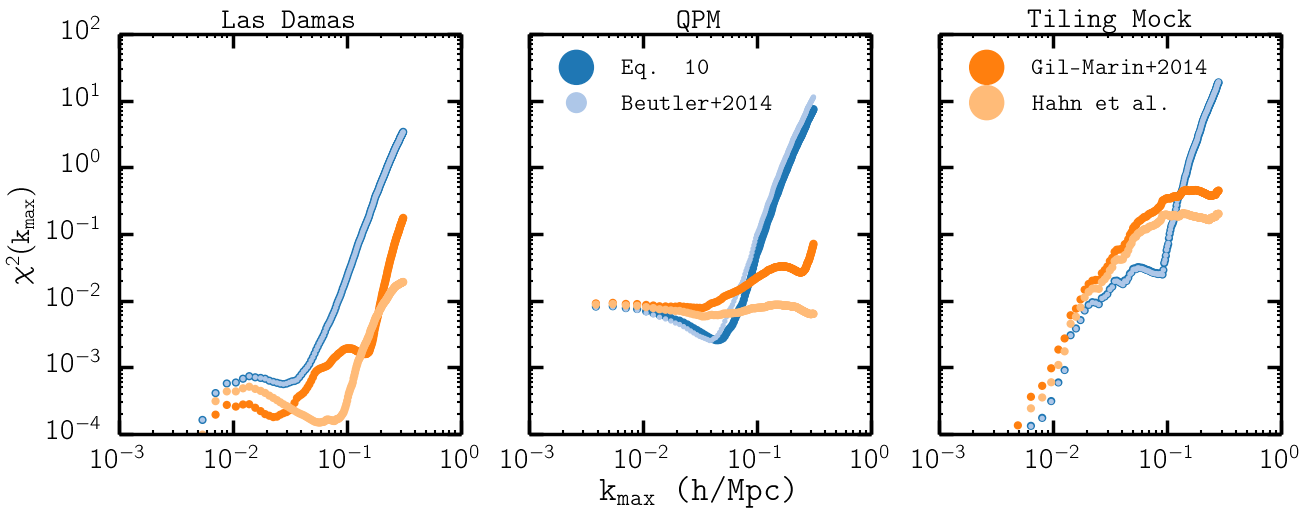
\includegraphics[scale=0.55]{fcpaper_pk_chisquared_comparison.png} 
\caption{$\chi^2 (k_\mathrm{max})$ for $P_\mathrm{NN-upweight}$ (blue), $P_\mathrm{Beutler}$ (light blue), $P_\mathrm{Gil-Marin}$ (orange), and $P_\mathrm{Hahn}$ (yellow) using the Las Damas (left panel), QPM (centerl panel), and Tiling (right panel) mock catalogues. Equation \ref{eq:chi2} was used to compute the $\chi^2(k_\mathrm{max})$. }\label{fig:peaksnchi2}
\end{center}
\end{figure*}

The correction method we present in this paper corrects for the effect of fiber-collisions to the extent where $P_\mathrm{corr}(k)$ measurements are no longer dominated by systematic effects at $k > 0.2 \; h/\mathrm{Mpc}$. With this in mind, we quantify the goodness-of-fit for all the corrected $P(k)$s to $P_\mathrm{true}(k)$ by comparing the the following $\chi^2$ to one another: 
\begin{equation}
\chi^2 (k_\mathrm{max}) = \frac{1}{N_{k_\mathrm{max}}} \sum\limits_{k< k_\mathrm{max}} \frac{(\overline{P_\mathrm{corr}(k)} - \overline{P_\mathrm{true}(k))^2}}{\Delta P_\mathrm{true} (k)^2}. \label{eq:chi2}
\end{equation}
$N_{k_\mathrm{max}}$ is the number of $k$ bins in the $P(k)$ calculation with $k < k_\mathrm{max}$. $\overline{P_\mathrm{corr}(k)}$ is the average fiber-collision corrected powerspectrum of all realizations for each catalogue. $\Delta P_\mathrm{true}(k)$ is the standard deviation of $P_\mathrm{true}(k)$ computed from all realizations of each mock catalogue. We calculate $\chi^2$ as a function of $k_\mathrm{max}$ in order to determine the accumulated $\chi^2$ to a specific scale ($k_\mathrm{max}$). In doing so, we determine the scale to which a power spectrum analysis can be extended to without suffering the significant effects of fiber-collisions. 

For the Tiling Mock catalogue, since there is only one realization, the variance ($\Delta P_\mathrm{true} (k)$) cannot be computed independently. However, for an estimate of the $\chi^2$, we use $\Delta P_\mathrm{true}^\mathrm{Tiling\;Mock}(k)$ from $\Delta P_\mathrm{true} (k)$ of the QPM mock catalogue scaled by the ratio of the power spectrum:
\begin{equation}
\Delta P_\mathrm{true}^\mathrm{Tiling}(k) = \Delta P_\mathrm{true}^{QPM}(k) \times \frac{P_\mathrm{true}^\mathrm{Tiling}(k)}{\overline{P^\mathrm{QPM}_\mathrm{true}(k)}}.
\end{equation}

In Figure \ref{fig:peaksnchi2}, we present the $\chi^2(k_\mathrm{max})$ for $P(k)$ using the following fiber collision correction methods: NN-upweight, \cite{Beutler:2014aa}, \cite{Gil-Marin:2014aa}, and our method from Section \ref{sec:apply}. The comparison is made using the Las Damas (left panel), QPM (center panel) and Tiling (right panel) mock catalogues. First in the Las Damas panel, at scales $k < 5 \times 10^{-2} \; h/\mathrm{Mpc}$, $\chi^2 < 10^{-3}$ for all correction methods, which suggests that all correction methods sufficiently correct for fiber-collisions and provide a reasonable fit to $P_\mathrm{true}(k)$ at these larger scale. In approaching smaller scales the $\chi^2$ for all correction methods increase. However, throughout the entire $k_\mathrm{max}$ range, our correction method provides a notably lower $\chi^2$ in comparison to the other correction methods. This is especially clear at $k \sim 0.3 \; h/\mathrm{Mpc}$, where $\chi^2_\mathrm{NN-upweight} \approx 0.33$, $\chi^2_\mathrm{Beutler} \approx 0.33$, and $\chi^2_\mathrm{Gil-Marin} \approx 0.17$ while $\chi^2 \approx 0.019$ for our method. 

Next in the central QPM panel, at large scales ($k < 2 \times 10^{-2} \; h/\mathrm{Mpc}$) all corrected $P(k)$ once again provide a reasonable reconstruction of $P_\mathrm{true}(k)$ with $\chi^2 \approx 10^{-2}$. Then for $2 \times 10^{-2} < k_\mathrm{max} < 5 \times 10^{-2}\; h/\mathrm{Mpc}$, NN-upweight and \cite{Beutler:2014aa} correction methods have the lower $\chi^2$s than \cite{Gil-Marin:2014aa} and our correction methods. However, at smaller scales, the $\chi^2$s of NN-upweight and \cite{Beutler:2014aa} quickly increase beyond the $\chi^2$s of \cite{Gil-Marin:2014aa} and our methods. Meanwhile, throughout the entire $k_\mathrm{max}$ range our correction method has a lower $\chi^2$ than the correction method of \cite{Gil-Marin:2014aa}. The difference in $\chi^2$ is again most remarkable at the smallest scales: $\chi^2 (k_\mathrm{max} \sim 0.3) \approx 7.3,\;11, \;0.068, \;\mathrm{and} \; 0.0063$ for NN-upweight, \cite{Beutler:2014aa}, \cite{Gil-Marin:2014aa} and our correction method respectively. 

Finally in the right panel (Tiling Mock), we find that $\chi^2(k_\mathrm{max})$ increases in a near monotonic fashion as a function of $k_\mathrm{max}$. For $k_\mathrm{max} < 4\times10^{-2} \; h/\mathrm{Mpc}$, there are no significant differences between the $\chi^2$s of all the correction methods. Then from $4\times10^{-2} < k_\mathrm{max} < 1.5\times 10^{-2} \; h/\mathrm{Mpc}$, $\chi^2$s of NN-upweight and \cite{Beutelr:2014aa} are notably lower than the $\chi^2$s of \cite{Gil-Marin:2014aa} and our method. However at smaller scales, the $\chi^2$s of NN-upweight and \cite{Beutelr:2014aa} quickly rise beyond the other $\chi^2$s, ultimately both reach $\chi^2(k_\mathrm{max} \sim 0.3) \approx 13.5$. In the meantime, $\chi^2(k_\mathrm{max} \sim 0.3) \approx 0.32$ for \cite{Gil-Marin:2014aa} and $\chi^2(k_\mathrm{max} \sim 0.3) \approx 0.15$ for our correction method. Moreover, through the entire $k_\mathrm{max}$ our method has a lower $\chi^2$ than \cite{Gil-Marin:2014aa}. With only one realization of the Tiling Mocks and scaled $\Delta P$, a detailed comparison of the $\chi^2$ values is impossible. Yet the $\chi^2(k_\mathrm{max})$ results for our correction provide realistic assurance that the correction method can be applied to the actually BOSS data.

Overall, regardless of catalogue, for scales $k_\mathrm{max} < 3 \times 10^{-2} \;h/\mathrm{Mpc}$, the $\chi^2$ for all fiber-collision corrected $P(k)$ are negligible. Then, with the exception of the Las Damas catalogue, at intermediate scales of $3 \times 10^{-2} < k_\mathrm{max} < 0.15 \; h/\mathrm{Mpc}$ the NN-upweight and \cite{Beutler:2014aa} methods show the lowest $\chi^2$s. At the smallest scales, however, these corrections methods no longer provide a good fit to $\overline{P_\mathrm{true}(k)}$. A detailed comparison at the small scales ($k > 1.5 \times 10^{-1} \;h/\mathrm{Mpc}$) demonstrates that the fiber-collision correction we present in this paper significantly better reproduces the true power spectrum than any of the other fiber-collision correction methods. Furthermore, Figure \ref{fig:peaksnchi2} illustrates that throughout the entire $k_\mathrm{max}$ is able to reasonably reproduces $P_\mathrm{true}(k)$ at all scales. 

% Detailed comparison to Gil-Marin that talk about how the xps value he calculates is only validated through mock catalogues, but our method can be validated with the overlapping regions of the real data. 

\section{Summary and Discussion} 
Using simulated mock catalogues for SDSS data with realistically imposed fiber-collisions, we quantify the systematic effects of fiber-collisions on galaxy clustering statistics, in particular the power spectrum. Although fiber-collisions have little significant effect on the power spectrum at large scales, its effect quickly overtakes the sample variance at scales smaller than $k \sim 0.1 \;h/\mathrm{Mpc}$. At the smallest scales that we explore in this paper, $k \sim 0.3$, fiber-collisions have over a $10 \%$ effect on the power spectrum. Consequently, at these small scales the uncertainties for power spectrum measurements are dominated by systematic effects from fiber-collisions. 

Fortunately, through the fiber-collided mock catalogues we are able to model the distribution of the line-of-sight displacement between fiber-collided pairs. Combining this model with a modified shot-noise term in the power spectrum estimator, we devise a new fiber-collision correction method that is able to reconstruct the true power spectrum from fiber-collided data even to $k \sim 0.3 \;h/\mathrm{Mpc}$. Throughout the entire $k$ range explored in our analysis, our correction method reconstructs $P_\mathrm{True}(k)$ safely within the sample variance. 

Furthermore, we compare our method to the most common nearest-neighbor correction method and recent correction methods presented in \cite{Beutler:2014aa} and \cite{Gil-Marin:2014aa} to demonstrate that our method most successfully reproduces the true power spectrum at small scales for all the Las Damas, QPM, and Tiling mock catalogues. As an added advantage, our correction method can also be validated by actual data rather than only through the mock catalogues thereby making it's application to actual data further reliable. 

The fiber-collision correction method we present will enable us to extend our galaxy clustering analysis to smaller scales for SDSS-III BOSS and future surveys such as eBOSS or any other large fiber-fed surveys. Our fiber-collision correction method can also be extend to higher order clustering statistics such as the bispectrum, which we will explore in future work. 

\bigskip
We thank something something

% No need for different sections, just present the different results 
\bibliographystyle{apj}
\bibliography{fc_paper}
\end{document}